\chapter{Research}
%\emph{This chapter reports on the execution of the research method as described in an earlier chapter. If the research has been divided into phases, they are introduced, reported on and concluded individually. If needed, this chapter could be split up to balance out the sizes of all chapters.}
This chapter reports on the execution of the research to demonstrate what has been done. First we explain the current difficulties with managing virtual networks on \gls{dcos}. Next we explore the approach how another popular container orchestration platform, Kubernetes, handles virtual networks. Last we explain the approach we took to build the \gls{poc}.

\section{Current state of virtual networks in DC/OS}
\Gls{dcos} provides virtual networks by itself as overlay networks which can be used by the Docker and Mesos containerizer. This overlay is prepacked and enabled by default on the cluster. \Gls{cni} plugins are also supported on \gls{dcos} and can be used by both containerizers.

\subsection{DC/OS virutal networks}
The overlay network was introduced to enable an IP-per-container model in \gls{dcos}. This allows operators to run applications on the default ports without worrying about port conflicts. This is done by creating an overlay network using \gls{vxlan}\cite{mahalingam2014virtual} which is supported by the Linux kernel. It works by creating two network bridges on each host, one for each containerizer. Containers on the same host and bridge can communicate directly with each other over the network bridge. And a packet from a Mesos container to a Docker container will be routed through both bridges. A packet from a Mesos container on Agent~1 to a Docker container on Agent~2 follows a different path. First the packet will be routed to the Mesos bridge, the host's network stack consumes the package and encapsulates using \gls{vxlan} on Agent~1. Next Agent~2 decapsulates this packet and sends it up to the Docker bridge to be sent to the Docker container as can be seen in Figure~\ref{fig:dcos-overlay-arch}.

IP address are managed by the agent itself instead of a central location. A central location requires a reliably and consistent way of handing IP addresses in the cluster. The default configuration uses a \texttt{9.0.0.0/8} subnet, this will devided in smaller chunks, a \texttt{/24} to be managed by every agent itself. On the agent this subnet is divided into two equal subnets for each containerizer, resulting in 32 usable IP addresses for each container type on every agent.
\begin{figure}
    \centering
    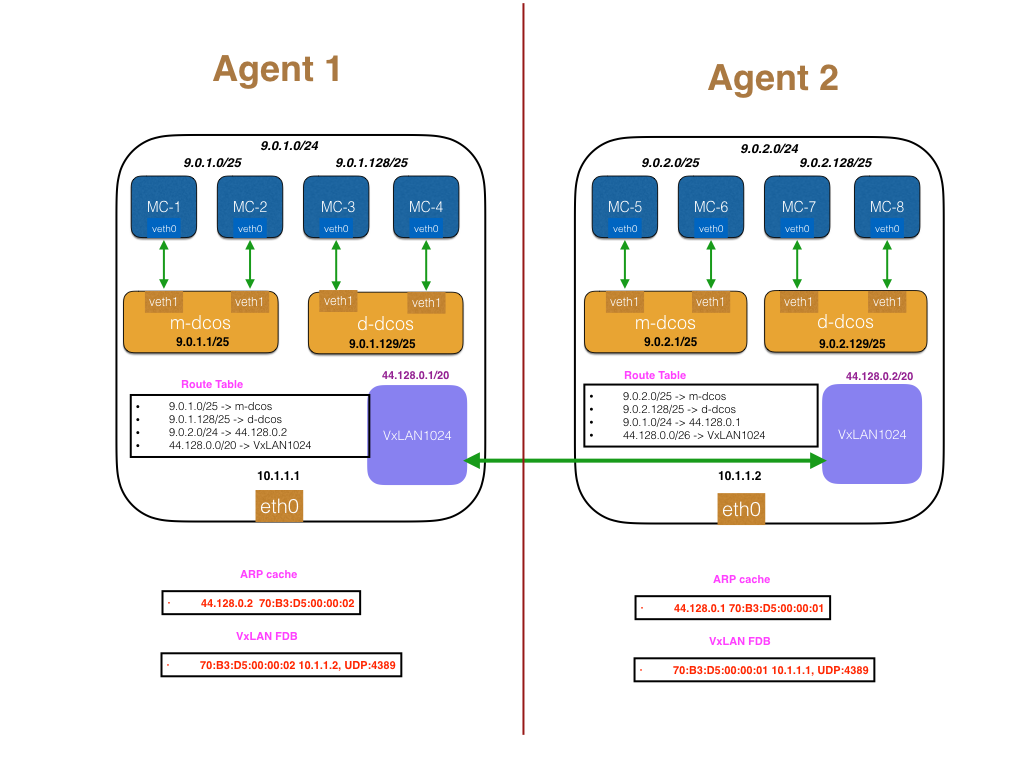
\includegraphics[width=1\columnwidth]{images/dcos-overlay-arch}
    \caption{DC/OS overlay in action\cite{dcos_overlay_arch}}
    \label{fig:dcos-overlay-arch}
\end{figure}

The default overlay network has the following limitations:
\begin{itemize}
    \item A limit on the number of usable IP addresses on each host, determined by the network prefix size. The default maximum is 32 Mesos and 32 Docker containers.
    \item Only IPv6 support for Docker containers, Mesos containers will fail to start.
    \item Operators are only able to create virtual networks during installation, this requires planning on before hand.
    \item The length of network names is limited as the Linux kernel only allows 15 characters for a network interface name.
    \item Marathon cannot execute healhtchecks in the default configurations as Marathon itself is not running on the virtual network.
\end{itemize}

\subsection{CNI plugins on DC/OS}
Too allow for more flexibility with virtual networks operators can also chose to create network with other providers.
\begin{displayquote}
    ``NOTE: The network tab currently displays information about containers that are associated with virtual networks managed by DC/OS overlay. It does not have information about containers running on virtual networks managed by any other CNI/CNM provider.'' %https://docs.mesosphere.com/1.11/networking/SDN/dcos-overlay/#limitations
\end{displayquote}



\subsection{Problems}

\section{Virtual networks in Kubernetes}

\section{Proof of concept}
